\section{Top Level Schematic}

\textit{\hyperlink{schematic.1}{schematic}}

The top level sheet instantiates the various subcomponents of the design. Additionally, it generates
a 40MHz clock signal that feeds into a clock buffer and is output to various components, as shown in
Figure~\ref{fig:clock-generator}. The LP5907 is a voltage regulator that takes a 3.6V input signal
generated by a buck converter on the power sheet and outputs a 1.8V signal to power the
\href{https://media.digikey.com/pdf/Data\%20Sheets/AVX\%20PDFs/KT2520K40000DAW18TAS_Spec.pdf}{KT2520K}
crystal oscillator which generates a 40MHz clock signal. The coupling capacitor attached in series to
the output of the crystal oscillator will prevent a DC bias from leaving the crystal oscillator. The
Schmitt inverter is used to turn the clipped sine wave output of the crystal oscillator into a
square wave. By connecting the output of the Schmitt inverter back to its input via two resistors
with a bypass capacitor between them, the input sine wave to the trigger becomes centered around
VCC/2, or 1.65V in this case. The capacitor filters out the high frequency signals centers it just at
the DC bias level. The 40MHz square wave feeds into the clock fanout buffer
\href{http://www.onsemi.com/pub/Collateral/NB3N551-D.PDF}{NB3N551} which generates 3 clock outputs
that oscillate at 40 MHz between about 0V and 3V.

\begin{figure}[h]
  \centering
  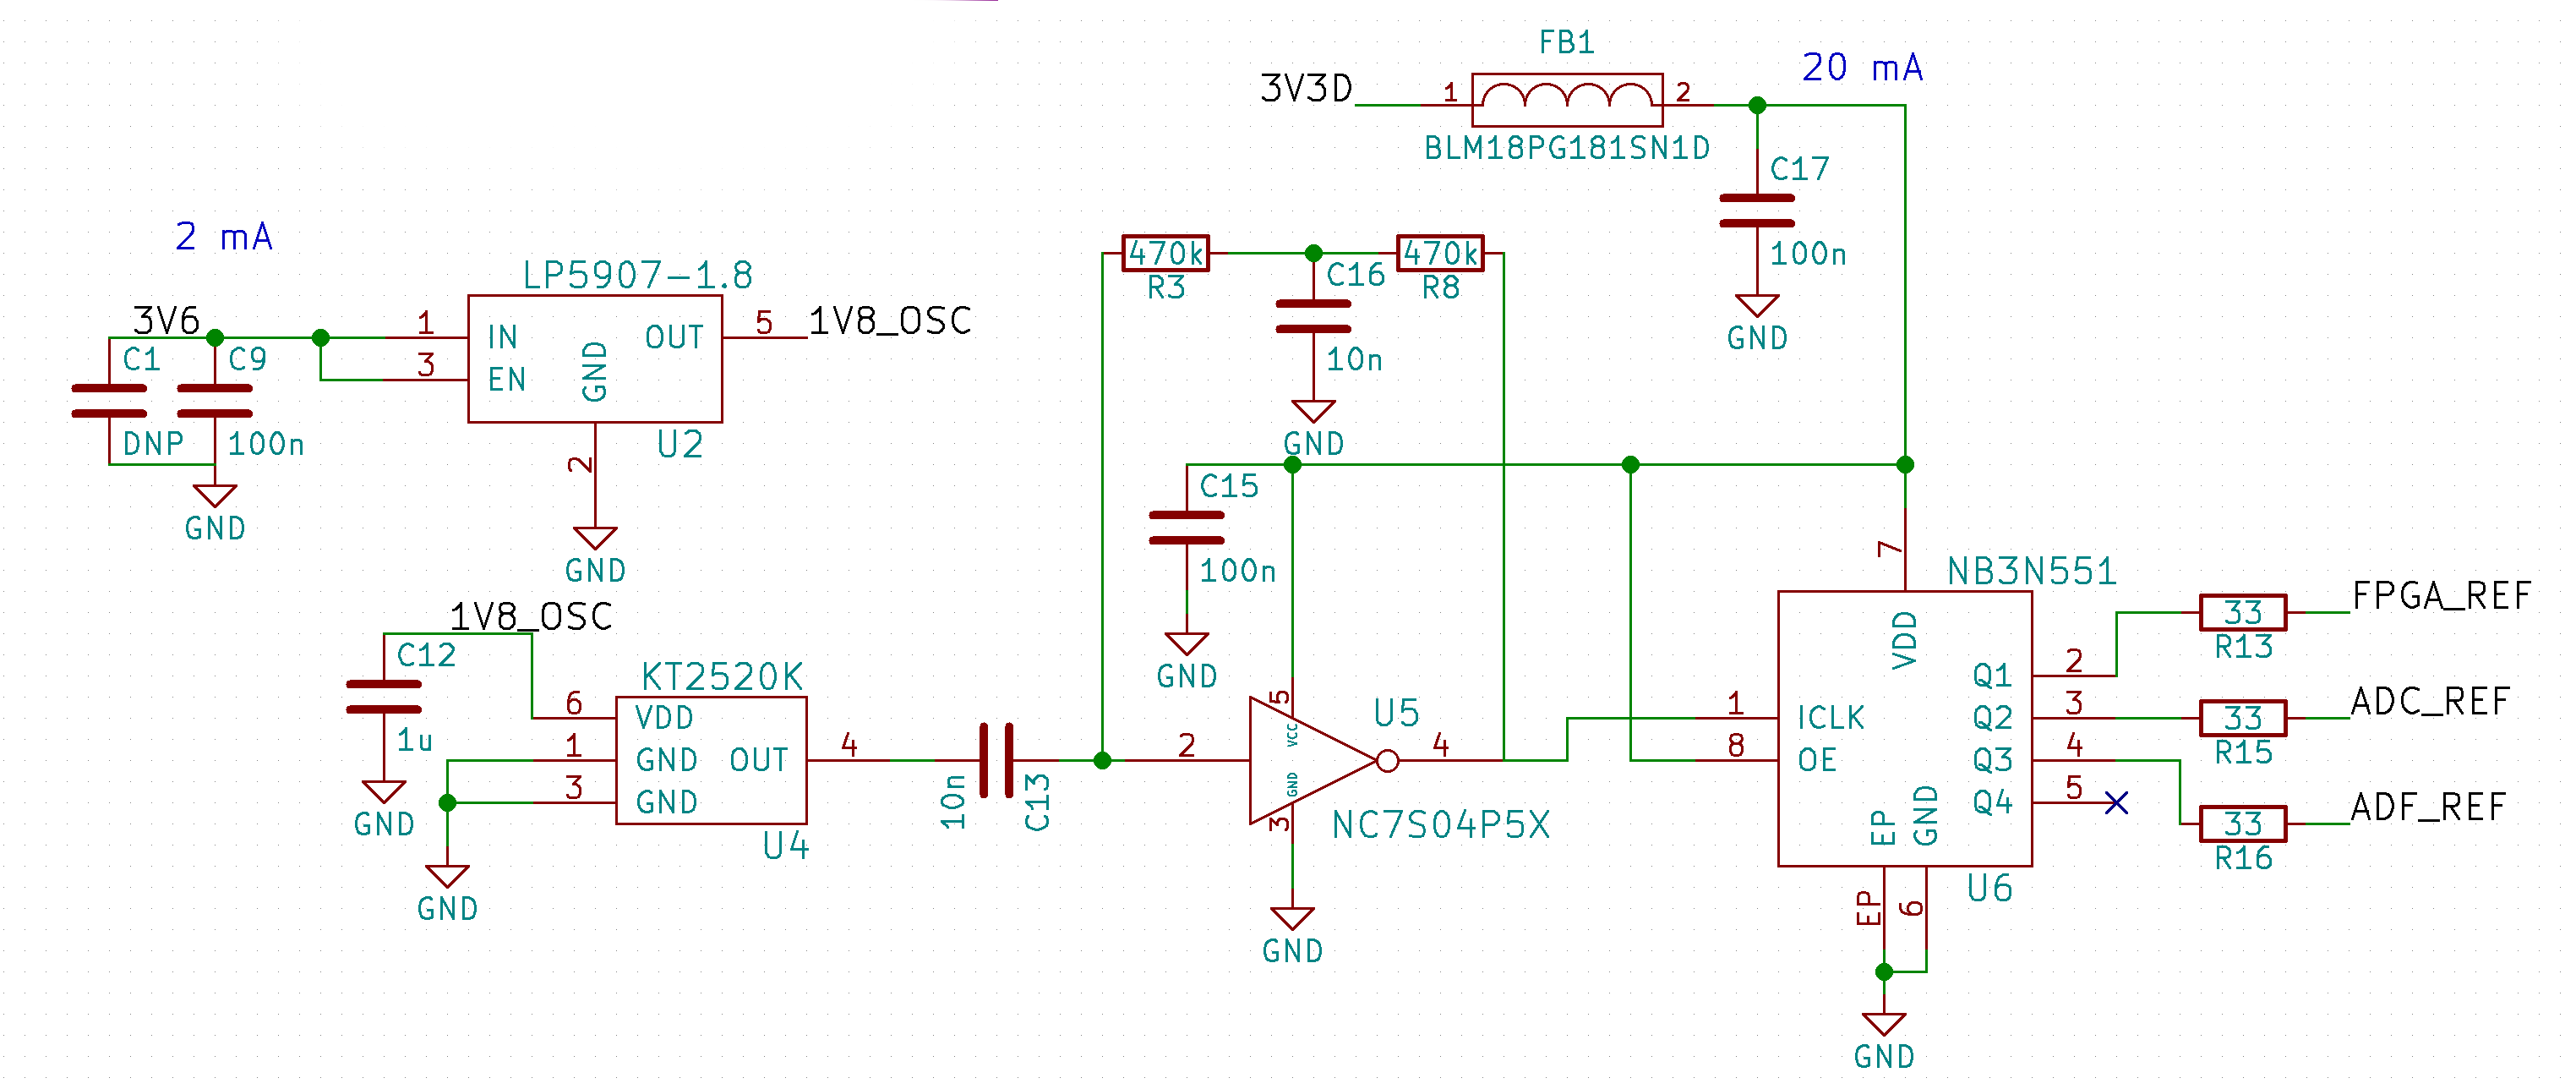
\includegraphics[width=1.0\textwidth]{data/clock-generator.png}
  \caption{A 40MHz clock signal is used to synchronize different components on the board.}
  \label{fig:clock-generator}
\end{figure}